\section{Simulation Infrastructure}\label{sec:ch3gemc}
    \subsection{Motivation for massive simulations}
    \subsection{OSG, MIT Tier 2, submission pipeline}

    Simulation hours: 
    As for your question, if there is constant pressure then yes, MIT baseline would be constant.

However: need much more than ~20K jobs / day to be at constant pressure. The dedicated resources + high priority can go up to 20K cores at once and if a job last 4 hours that’s 24/4 = 6*20K = 120K jobs / day to be at constant pressure! Please do not submit that many jobs ;-)

You can check the monitoring page for more details. In particular you can select 1 month timeframe, and log scale. You will see holes in queue.
And if you select just ‘MIT’ on the dedicated graph, you’ll see the attached picture, where the ‘holes’ in the pressure are well shown and the number of MIT cores under pressure is about 3K.

Xiaqing said that the following: \cite{Dreschsel1992ThresholdNucleons} contains the formalism for the MAID model


\section{Generator Details}\label{sec:ch3generator}
    \subsection{AAO}
        \subsection{AAONORAD}
        \subsection{AAORAD}

\section{Simulation Pipeline}
    \section{GEMC}

\section{Investigation into Simulation Speedup: Normalizing Flows}


\section{Getting Started}
    Dear Andrey,
    
    Could you send us a link to the github for aao\_rad and aao\_norad with some instructions so that Bobby can follow up for his pi0 analysis?  
    
    Dear Bobby,
    
    aao\_rad and aao\_norad are event generators for exclusive pi0 and pi+ channels with/without radiative effects.  They are written in Fortran.  The program was initially developed by Volker Burkert long time ago for the resonance region, then has been evolved for many years and recently extended to DIS region even though lots of things need to be done.  Try this to see whether it works.  
    
    Thanks.
    
    Best regards, Kyungseon
    
    
    Dear Stefan,
    
    Could you upload the program (C++ version, perhaps in Githup with some instructions) that Kemal Tezgin recently wrote in order to calculate the pi0/pi+ channel observables based on the most recent GK model calculations?  Thanks.
    
    Best regards, Kyungseon
    
    
    Dear Kyungseon,
    
    I have attached the program to calculate the single terms of the pi0 
    cross-section based on the GK model.
    Its only one file and relatively easy to use. The instructions are in 
    the first few rows of the file.
    The output can be modified in the main routine at the end of the file.
    
    Best regards,
    Stefan --- this file is name Pi\_GK\_Vegas.cpp
    
    
    Hi Bobby,
    Please take a look at README:
    \href{https://github.com/drewkenjo/aao\_norad}{norad}
    It has instructions how to compile, run and configure the program.
    Please don't hesitate to ask questions!
    Best,
    Andrey.
    need make an initial cut on photon energies
use aao\_rad or no\_rad etc. to define what energy is needed for photon energy cut

\section{More notes}
    

    For event generator we have aao\_rad can generate radiatied pi0 events in resoncane region use 2007 model
    Put parameterization from valerly’s paper, can cover up to whatever Q2 range covered in the paper, beyond that we put some general Q2 behaviour
    For Exclurad we have similar model, in end may have to iterate a few times to improve the model
    Exlclurad specifically for resonance region, theoretically should be correct, input probably needs to be updated, can put Valery’s new parameterization to cover higher range. Should not be a real issue to implement it because same thing was done for AAORad. High q2 cannot be covered because parameterization only goes to CLAS6 range
    FX: the cruicail thing is to fold in the radiative corrections with acceptance and efficiens. Best mothod is to use fast monte carlo




\section{Generator}
Generator Notes:
You don't need much details about generator, it is based on GK model with Valery's fit to CLAS6 data.

NON RADIATED, INBENDING
// Pi0 leptoproduction in Goloskokov-Kroll (GK) model. The code is currently being tested and implemented in PARTONS framework with additional features. If you plan to use this work in a publication, please use and reference the most recent version of PARTONS in http://partons.cea.fr 

the gk model is fit from clas6 data?

I have a couple questions:

Andrey Kim and Nick Markov have the pi0 generator. It has my parametrization for W>2 GeV and MAID for W<1.7 GeV.

My model will for sure work for 12 GeV. It actually very close even for the COMPASS pi0 data (180 GeV muon beam).

There is reasonable coincidence between my model and MAID in the point W=1.7 GeV, not ideal but good enough for the MC.

I think actually that my parametrization has to work in the region W<2 GeV but I am not sure that MAID is doing good job due to the absence the experimental data at W~1.7 GeV. 





\iffalse
NOTES TO SELF:
physics motivation
data sets before event selection
PID
exclusive cuts
results to show
1 slide of what needs to go from here to cross section
\fi

\section{Generator and Simulations}
    Simulations are necessary in order to extract correction factors. Presently, only an acceptance correction using a non-radiative generator has been calculated; other correction factors are forthcoming but will not be including in this note. 

    GEMC was used to process generated events through the CLAS12 fall 2018 RG-A configuration. Specifically, a generator based off the GK model and CLAS6 data - aao\_norad\footnote{https://github.com/drewkenjo/aao\_norad}. 
    

\section{Comparison to Data: Missing Mass Distributions}

The standard aao simulations result in missing mass distributions that are too optimistic compared to experimental data. Observe the discrepancies between simulated and experimental distributions in figure \ref{fig:bad}. 


\begin{figure}[hbt]
	\centering
	\includegraphics[page=125,width=0.3\linewidth]{Chapters/Ch3-Simulations/pics/nosmear/outbending_rad_All_All_All_no_smearingME_epgg_exp_vs_sim.png}
	\includegraphics[page=123,width=0.3\linewidth]{Chapters/Ch3-Simulations/pics/nosmear/outbending_rad_All_All_All_no_smearingMM2_egg_exp_vs_sim.png}
	\includegraphics[page=128,width=0.3\linewidth]{Chapters/Ch3-Simulations/pics/nosmear/outbending_rad_All_All_All_no_smearingMM2_epgg_exp_vs_sim.png}
	\includegraphics[page=130,width=0.3\linewidth]{Chapters/Ch3-Simulations/pics/nosmear/outbending_rad_All_All_All_no_smearingMM2_ep_exp_vs_sim.png}
	\includegraphics[page=133,width=0.3\linewidth]{Chapters/Ch3-Simulations/pics/nosmear/outbending_rad_All_All_All_no_smearingMpi0_exp_vs_sim.png}
	\includegraphics[page=135,width=0.3\linewidth]{Chapters/Ch3-Simulations/pics/nosmear/outbending_rad_All_All_All_no_smearingMPt_exp_vs_sim.png}
	
	\caption{Comparison of experiment (blue) and simulation (red) missing mass, energy, momentum, and invariant gamma-gamma mass distributions, before any smearing factors were added to the simulation data.}
	\label{fig:bad}
\end{figure}



To improve the matching between simulation and experiment, gaussian smearing factors were added after reconstruction to the simulated dataset. These factors were tuned by Sangbaek Lee to have optimal matching across all missing mass spectra combinations (figure \ref{fig:good}. Once these factors were determined, the simulations were used to extract an acceptance correction.


\begin{figure}[hbt]
	\centering
	\includegraphics[page=125,width=0.3\linewidth]{Chapters/Ch3-Simulations/pics/yessmear/outbending_rad_All_All_All_for_aps_2022_plots_sangcutsME_epgg_exp_vs_sim.png}
	\includegraphics[page=123,width=0.3\linewidth]{Chapters/Ch3-Simulations/pics/yessmear/outbending_rad_All_All_All_for_aps_2022_plots_sangcutsMM2_egg_exp_vs_sim.png}
	\includegraphics[page=128,width=0.3\linewidth]{Chapters/Ch3-Simulations/pics/yessmear/outbending_rad_All_All_All_for_aps_2022_plots_sangcutsMM2_epgg_exp_vs_sim.png}
	\includegraphics[page=130,width=0.3\linewidth]{Chapters/Ch3-Simulations/pics/yessmear/outbending_rad_All_All_All_for_aps_2022_plots_sangcutsMM2_ep_exp_vs_sim.png}
	\includegraphics[page=133,width=0.3\linewidth]{Chapters/Ch3-Simulations/pics/yessmear/outbending_rad_All_All_All_for_aps_2022_plots_sangcutsMpi0_exp_vs_sim.png}
	\includegraphics[page=135,width=0.3\linewidth]{Chapters/Ch3-Simulations/pics/yessmear/outbending_rad_All_All_All_for_aps_2022_plots_sangcutsMPt_exp_vs_sim.png}
	
	\caption{Comparison of experiment (blue) and simulation (red) missing mass, energy, momentum, and invariant gamma-gamma mass distributions, with smearing factors added to the simulation data proton and photon momenta.}
	\label{fig:good}
\end{figure}


\section{Acceptance Correction}

The acceptance correction, in each kinematic bin, was simply calculated as $\frac{N_{rec}}{N_{gen}}$, where $N_{gen}$ is the number of events produced by the generator in a specific bin, and $N_{rec}$ is the number of events in that bin that were reconstructed and identified as a $DV\pi^0P$ event by exclusivity cuts. 

Low acceptance bins (less than 5\%) were excluded from further study, following from the CLAS6 analysis procedure. 